\documentclass[tikz,border=3pt]{standalone}
% Shared preamble for the standalone TikZ diagrams (included after \documentclass).
% Build with build.sh. Language is selected with \def\VI{1} (Vietnamese) or by default English:
%   \LL{English text}{Văn bản tiếng Việt}
\usepackage{fontspec}
\IfFontExistsTF{Times New Roman}{\setmainfont{Times New Roman}}{%
  \setmainfont{times.ttf}[Path=/mnt/c/Windows/Fonts/,
    BoldFont=timesbd.ttf,ItalicFont=timesi.ttf,BoldItalicFont=timesbi.ttf]}
\usepackage{xcolor}
\usepackage{tikz}
\usetikzlibrary{arrows.meta,positioning,calc,fit,backgrounds,patterns,shapes.misc,decorations.pathreplacing}

\newcommand{\LL}[2]{\ifdefined\VI #2\else #1\fi}
\hyphenpenalty=10000 \exhyphenpenalty=10000 \tolerance=9999 \emergencystretch=3em

% --- palette (print-safe: meaning is never carried by colour alone) -----------
\definecolor{ink}{HTML}{1F2937}
\definecolor{muted}{HTML}{6B7280}
\definecolor{rule}{HTML}{9CA3AF}
\definecolor{shfill}{HTML}{DCE8F5}   % shared
\definecolor{shline}{HTML}{2F5D8C}
\definecolor{dedfill}{HTML}{FBE5CF}  % dedicated
\definecolor{dedline}{HTML}{B5651D}
\definecolor{neutral}{HTML}{F3F4F6}
\definecolor{appfill}{HTML}{F6F9FC}
\definecolor{appline}{HTML}{7C93AD}
\definecolor{ctlfill}{HTML}{EFEAF7}
\definecolor{ctlline}{HTML}{6B5B95}
\definecolor{warn}{HTML}{B91C1C}
\definecolor{ta}{HTML}{2A9D8F}       % tenant A
\definecolor{tb}{HTML}{E09F3E}       % tenant B
\definecolor{tc}{HTML}{8E6BBF}       % tenant C
\colorlet{taL}{ta!22}
\colorlet{tbL}{tb!28}
\colorlet{tcL}{tc!24}

\tikzset{
  >=Latex,
  every node/.style={font=\footnotesize, text=ink, inner sep=2pt},
  box/.style={draw=ink!65, rounded corners=1.6pt, line width=0.5pt, fill=white,
              align=center, inner sep=3pt, minimum height=5mm},
  shared/.style={box, fill=shfill, draw=shline},
  ded/.style={box, fill=dedfill, draw=dedline},
  plain/.style={box, fill=neutral, draw=rule},
  ta/.style={box, fill=taL, draw=ta},
  tb/.style={box, fill=tbL, draw=tb},
  tc/.style={box, fill=tcL, draw=tc},
  tenantA/.style={ta}, tenantB/.style={tb}, tenantC/.style={tc},
  zone/.style={draw=appline, fill=appfill, rounded corners=2.5pt, line width=0.6pt},
  ctlzone/.style={draw=ctlline, fill=ctlfill, rounded corners=2.5pt, line width=0.6pt},
  ttl/.style={font=\small\bfseries, text=ink, align=left, inner sep=1pt},
  cp/.style={font=\scriptsize, text=muted, align=center, inner sep=1pt},
  note/.style={font=\scriptsize, text=muted, align=left, inner sep=1pt},
  arr/.style={->, line width=0.6pt, draw=ink!80},
  arrm/.style={->, line width=0.6pt, draw=muted, dashed},
  link/.style={line width=0.5pt, draw=muted},
  bound/.style={line width=0.8pt, draw=warn, dash pattern=on 3pt off 2pt},
  badge/.style={circle, fill=ink, text=white, font=\scriptsize\bfseries, inner sep=1.2pt, minimum size=3.6mm},
}

% a small user glyph (head + shoulders) centred at the given coordinate, colour as 3rd arg

% user glyph: head and shoulders, centred at (x,y); 3rd argument = colour
\newcommand{\user}[3]{%
  \fill[#3] (#1,#2) circle (0.85mm);
  \fill[#3] ($(#1,#2)+(-1.5mm,-2.5mm)$) arc (180:0:1.5mm) -- cycle;}

% Figure: the selected architecture <AI, DB> (shared application instance, schema per tenant) with the
% policy-selected variants of the Bridge. Numbered guards 1-5 are the independent tenant-isolation checks.
\begin{document}
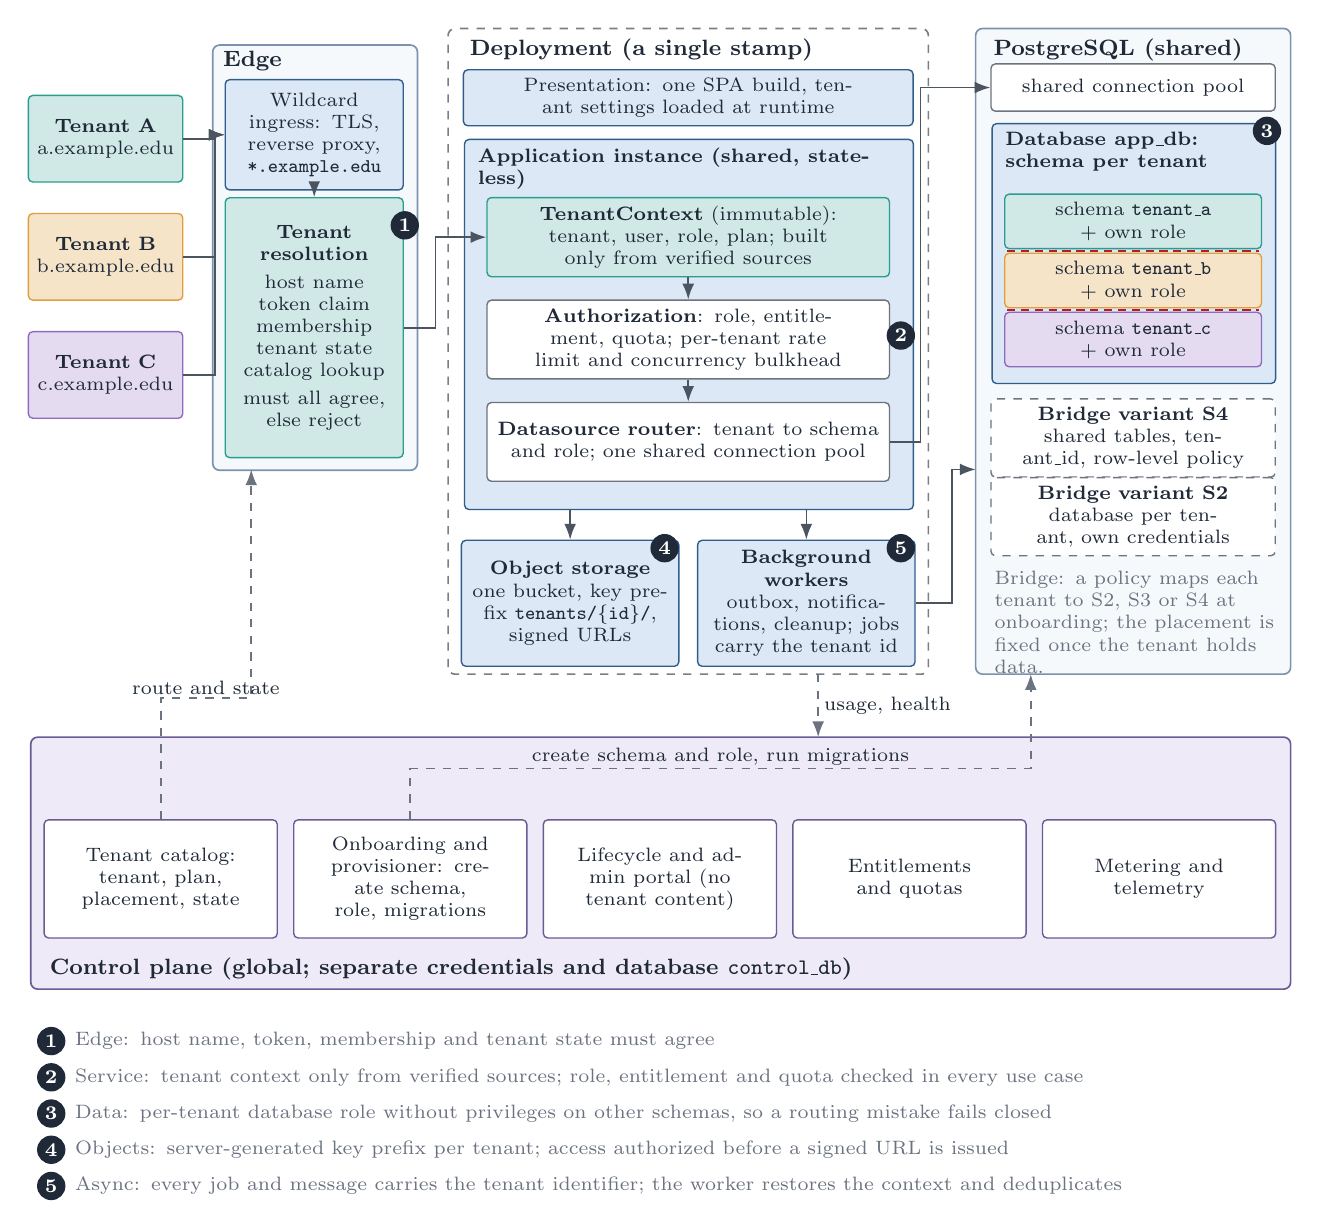
\begin{tikzpicture}[x=1mm,y=1mm]
\newcommand{\guard}[3]{\node[badge] at (#1,#2) {#3};}

% ============================================================= users and edge
\foreach \y/\c/\n/\h in {104/ta/A/a, 89/tb/B/b, 74/tc/C/c} {
  \node[\c,minimum width=19mm,minimum height=11mm,text width=17.5mm,font=\scriptsize] (u\n) at (9.5,\y) {\textbf{\LL{Tenant \n}{Thuê bao \n}}\\\h.example.edu};
}
\node[ctlzone,draw=appline,fill=appfill,minimum width=26mm,minimum height=54mm,anchor=north west] at (23,116) {};
\node[ttl,anchor=north west,font=\footnotesize\bfseries] at (24,115.6) {\LL{Edge}{Biên}};
\node[shared,minimum width=22mm,minimum height=14mm,text width=20.5mm,font=\scriptsize] (ing) at (36,104.5) {\LL{Wildcard ingress: TLS, reverse proxy, \texttt{*.example.edu}}{Lối vào ký tự đại diện: TLS, proxy ngược, \texttt{*.example.edu}}};
\node[box,fill=taL,draw=ta,minimum width=22mm,minimum height=33mm,text width=20.5mm,font=\scriptsize] (res) at (36,80) {\textbf{\LL{Tenant resolution}{Nhận diện thuê bao}}\\[2pt]\LL{host name\\token claim\\membership\\tenant state\\catalog lookup\\[2pt]must all agree, else reject}{tên miền\\định danh trong token\\tư cách thành viên\\trạng thái thuê bao\\tra danh mục\\[2pt]phải khớp, nếu không thì từ chối}};
\foreach \n in {A,B,C} { \draw[arr] (u\n.east) -- ($(u\n.east)+(4,0)$) |- (ing.west); }
\draw[arr] (ing) -- (res);
\guard{47.5}{93}{1}

% ============================================================= deployment frame
\draw[dashed,draw=ink!60,line width=0.6pt,rounded corners=2.5pt,fill=white] (53,36) rectangle (114,118);
\node[font=\footnotesize\bfseries,anchor=north west] at (55,117.4) {\LL{Deployment (a single stamp)}{Bản triển khai (một cụm duy nhất)}};
\node[shared,minimum width=57mm,minimum height=6.5mm,text width=55mm,font=\scriptsize] at (83.5,109.2) {\LL{Presentation: one SPA build, tenant settings loaded at runtime}{Trình diễn: một bản dựng SPA, cấu hình thuê bao nạp lúc chạy}};
% application instance
\node[shared,minimum width=57mm,minimum height=47mm,anchor=north west] (appz) at (55,104) {};
\node[font=\scriptsize\bfseries,anchor=north west,text width=54mm] at (56,103.6) {\LL{Application instance (shared, stateless)}{Thể hiện ứng dụng (dùng chung, không giữ trạng thái)}};
\node[box,fill=taL,draw=ta,minimum width=51mm,minimum height=10mm,text width=49mm,font=\scriptsize] (ctx) at (83.5,91.5) {\textbf{TenantContext} \LL{(immutable): tenant, user, role, plan; built only from verified sources}{(bất biến): thuê bao, người dùng, vai trò, gói; chỉ dựng từ nguồn đã xác minh}};
\node[box,fill=white,minimum width=51mm,minimum height=10mm,text width=49mm,font=\scriptsize] (auth) at (83.5,78.5) {\textbf{\LL{Authorization}{Phân quyền}}\LL{: role, entitlement, quota; per-tenant rate limit and concurrency bulkhead}{: vai trò, quyền sử dụng, hạn mức; giới hạn tốc độ và vách ngăn đồng thời theo thuê bao}};
\node[box,fill=white,minimum width=51mm,minimum height=10mm,text width=49mm,font=\scriptsize] (rtr) at (83.5,65.5) {\textbf{\LL{Datasource router}{Bộ định tuyến nguồn dữ liệu}}\LL{: tenant to schema and role; one shared connection pool}{: thuê bao tới lược đồ và role; một nhóm kết nối dùng chung}};
\draw[arr] (ctx) -- (auth);
\draw[arr] (auth) -- (rtr);
\guard{110.5}{79}{2}
% object storage (left) and workers (right) inside the deployment
\node[shared,minimum width=27mm,minimum height=16mm,text width=25.5mm,font=\scriptsize] (obj) at (68.5,45) {\textbf{\LL{Object storage}{Lưu trữ đối tượng}}\\\LL{one bucket, key prefix \texttt{tenants/\{id\}/}, signed URLs}{một bucket, tiền tố khóa \texttt{tenants/\{id\}/}, URL ký}};
\node[shared,minimum width=27mm,minimum height=16mm,text width=25.5mm,font=\scriptsize] (wrk) at (98.5,45) {\textbf{\LL{Background workers}{Tiến trình nền}}\\\LL{outbox, notifications, cleanup; jobs carry the tenant id}{outbox, thông báo, dọn dẹp; tác vụ mang định danh thuê bao}};
\draw[arr] (68.5,57) -- (obj.north);
\draw[arr] (98.5,57) -- (wrk.north);
\guard{80.5}{52}{4}
\guard{110.5}{52}{5}
% edge to application
\draw[arr] (res.east) -- (51.4,80) -- (51.4,91.5) -- (ctx.west);

% ============================================================= data layer
\draw[zone,fill=appfill] (120,36) rectangle (160,118);
\node[font=\footnotesize\bfseries,anchor=north west,text width=38mm] at (121.5,117.4) {\LL{PostgreSQL (shared)}{PostgreSQL (dùng chung)}};
\node[box,fill=white,minimum width=36mm,minimum height=6mm,text width=34mm,font=\scriptsize] (pool) at (140,110.5) {\LL{shared connection pool}{nhóm kết nối dùng chung}};
\node[shared,minimum width=36mm,minimum height=33mm,anchor=north west] (appdb) at (122,106) {};
\node[font=\scriptsize\bfseries,anchor=north west,text width=30mm] at (123,105.6) {\LL{Database app\_db: schema per tenant}{CSDL app\_db: lược đồ riêng mỗi thuê bao}};
\foreach \y/\c/\s in {93.5/ta/a, 86/tb/b, 78.5/tc/c} {
  \node[\c,minimum width=32mm,minimum height=6.5mm,text width=30.5mm,font=\scriptsize] at (140,\y) {\LL{schema \texttt{tenant\_\s} + own role}{lược đồ \texttt{tenant\_\s} + role riêng}};
}
\draw[bound] (124,89.75) -- (156,89.75);
\draw[bound] (124,82.25) -- (156,82.25);
\guard{157}{105}{3}
\node[box,dashed,fill=white,minimum width=36mm,minimum height=9mm,text width=34mm,font=\scriptsize] (v4) at (140,66) {\textbf{\LL{Bridge variant S4}{Biến thể S4 của Bridge}}\\\LL{shared tables, tenant\_id, row-level policy}{bảng chung, tenant\_id, chính sách mức dòng}};
\node[box,dashed,fill=white,minimum width=36mm,minimum height=9mm,text width=34mm,font=\scriptsize] (v2) at (140,56) {\textbf{\LL{Bridge variant S2}{Biến thể S2 của Bridge}}\\\LL{database per tenant, own credentials}{CSDL riêng mỗi thuê bao, thông tin đăng nhập riêng}};
\node[note,anchor=north west,text width=36mm] at (122,49.5) {\LL{Bridge: a policy maps each tenant to S2, S3 or S4 at onboarding; the placement is fixed once the tenant holds data.}{Bridge: chính sách gán mỗi thuê bao vào S2, S3 hoặc S4 lúc đăng ký; vị trí cố định khi thuê bao đã có dữ liệu.}};
\draw[arr] (rtr.east) -- (113,65.5) -- (113,110.5) -- (pool.west);
\draw[arr] (wrk.east) -- (117,45) -- (117,62) -- (120,62);

% ============================================================= control plane
\draw[ctlzone] (0,-4) rectangle (160,28);
\node[ttl,anchor=south west,text width=156mm,font=\footnotesize\bfseries] at (2,-3.3) {\LL{Control plane (global; separate credentials and database \texttt{control\_db})}{Mặt phẳng điều khiển (toàn cục; thông tin đăng nhập riêng và CSDL \texttt{control\_db})}};
\foreach \i/\en/\vi in {
  0/{Tenant catalog: tenant, plan, placement, state}/{Danh mục thuê bao: thuê bao, gói, vị trí, trạng thái},
  1/{Onboarding and provisioner: create schema, role, migrations}/{Đăng ký và bộ cấp phát: tạo lược đồ, role, migration},
  2/{Lifecycle and admin portal (no tenant content)}/{Vòng đời và cổng quản trị (không xem nội dung thuê bao)},
  3/{Entitlements and quotas}/{Quyền sử dụng và hạn mức},
  4/{Metering and telemetry}/{Đo lường và giám sát}} {
  \node[box,fill=white,draw=ctlline,minimum width=29mm,minimum height=15mm,text width=27.5mm,font=\scriptsize] (cp\i) at (16.5+\i*31.7,10) {\LL{\en}{\vi}};
}
% control plane to application plane
\draw[arrm] (cp0.north) -- (16.5,33) -- node[pos=0.5,above,note,text=ink] {\LL{route and state}{định tuyến, trạng thái}} (28,33) -- (28,62);
\draw[arrm] (cp1.north) -- (48.2,24) -- node[pos=0.5,above,note,text=ink] {\LL{create schema and role, run migrations}{tạo lược đồ và role, chạy migration}} (127,24) -- (127,36);
\draw[arrm] (100,36) -- node[right=0.3mm,note,text=ink,pos=0.5] {\LL{usage, health}{sử dụng, tình trạng}} (100,28);

% ============================================================= legend of guards
\foreach \y/\n/\en/\vi in {
  -10.6/1/{Edge: host name, token, membership and tenant state must agree}/{Biên: tên miền, token, tư cách thành viên và trạng thái thuê bao phải khớp},
  -15.2/2/{Service: tenant context only from verified sources; role, entitlement and quota checked in every use case}/{Dịch vụ: ngữ cảnh thuê bao chỉ từ nguồn đã xác minh; kiểm tra vai trò, quyền sử dụng, hạn mức ở mọi ca sử dụng},
  -19.8/3/{Data: per-tenant database role without privileges on other schemas, so a routing mistake fails closed}/{Dữ liệu: role CSDL riêng, không có quyền trên lược đồ khác, nên lỗi định tuyến bị từ chối thay vì lộ dữ liệu},
  -24.4/4/{Objects: server-generated key prefix per tenant; access authorized before a signed URL is issued}/{Đối tượng: tiền tố khóa do máy chủ tạo theo thuê bao; phân quyền trước khi cấp URL ký},
  -29/5/{Async: every job and message carries the tenant identifier; the worker restores the context and deduplicates}/{Bất đồng bộ: mọi tác vụ và thông điệp mang định danh thuê bao; tiến trình nền khôi phục ngữ cảnh và chống xử lý trùng}} {
  \node[badge] at (2.6,\y) {\n};
  \node[note,anchor=west,text width=150mm] at (5.2,\y) {\LL{\en}{\vi}};
}

\end{tikzpicture}
\end{document}
